\documentclass[aspectratio=169,11pt]{beamer}

\usepackage[utf8]{inputenc}
\usepackage[T1]{fontenc}
\usepackage[spanish]{babel}
\usepackage{amsmath,amssymb}
\usepackage{tikz}
\usetikzlibrary{arrows.meta,angles}

\usetheme{Madrid}
\usecolortheme{default}
\setbeamertemplate{navigation symbols}{}
\setbeamertemplate{blocks}[rounded][shadow=false]

\newcommand{\ang}[1]{\angle #1^\circ}

\title[Funciones de transferencia]{Paso 2: Funciones de transferencia, polos y ceros}
\subtitle{De la ecuación diferencial a $P(s)$}
\author{Curso de control robusto (QFT)}
\date{}

\begin{document}

% ------------------------------------------------------------
\begin{frame}
  \titlepage
\end{frame}

% ------------------------------------------------------------
\begin{frame}{Dónde encaja este paso}
  \tiny
  \begin{enumerate}\setlength{\itemsep}{-2pt}
    \item[1.] Números complejos \hfill \textcolor{gray}{(hecho)}
    \item[\textbf{2.}] \textbf{Funciones de transferencia: $s$, polos y ceros} \hfill $\leftarrow$ estamos aquí
    \item[3.] Respuesta en frecuencia: $s=j\omega$, magnitud y fase
    \item[4.] Decibelios y escala logarítmica (Bode)
    \item[5.] Realimentación: $L$, $T=\frac{L}{1+L}$, $S=\frac{1}{1+L}$
    \item[6.] Nichols chart
    \item[7.] Incertidumbre y templates
    \item[8.] Especificaciones $\rightarrow$ bounds
    \item[9.] Loop shaping, prefiltro y verificación
    \item[10.] QFT en control digital
    \item[11.] Dos caminos digitales: $z$ y $w$
    \item[12.] Estabilidad, límites, más especificaciones y caso real
    \item[13.] Muestreo por eventos con periodo base $T$
    \item[14.] Sistemas de dos estados: lazo interno y externo
    \item[15.] QFT y sistemas no lineales
    \item[16.] Algoritmos de QFT: cómo funcionan por dentro
    \item[17.] QFT en Python: una biblioteca paso a paso
    \item[18.] QFT en MATLAB: el mismo código, otra sintaxis
    \item[19.] Historia, panorama y bibliografía
  \end{enumerate}
  \vspace{0pt}
  \begin{block}{Objetivo de hoy}
    Entender de dónde sale $P(s)=\dfrac{1}{(s+5)(s+30)}$, qué son sus \textbf{polos y ceros}, y por qué $P(j\omega)$ (el paso 1) es solo $P(s)$ en $s=j\omega$.
  \end{block}
\end{frame}

% ------------------------------------------------------------
\begin{frame}{Un sistema: algo que transforma una entrada en una salida}
  \centering
  \begin{tikzpicture}[>=Stealth, node distance=3.2cm]
    \node[draw, rounded corners, minimum width=3.4cm, minimum height=1.3cm, fill=blue!8] (P) {Sistema $P$};
    \draw[->, thick] (-3.8,0) -- node[above]{entrada $u(t)$} (P.west);
    \draw[->, thick] (P.east) -- node[above]{salida $y(t)$} (3.8,0);
  \end{tikzpicture}

  \vspace{6pt}
  \begin{columns}[T]
    \begin{column}{0.48\textwidth}
      \begin{block}{Ejemplos}
        \small
        \begin{itemize}
          \item Motor: tensión $\to$ velocidad.
          \item Vehículo: par en la rueda $\to$ velocidad.
          \item Calefactor: potencia $\to$ temperatura.
        \end{itemize}
      \end{block}
    \end{column}
    \begin{column}{0.48\textwidth}
      \begin{block}{Qué supondremos: sistema lineal e invariante (LTI)}
        \small
        Lineal: si la entrada se duplica, la salida se duplica. Invariante: se comporta igual hoy que mañana. QFT trabaja con esta clase de sistemas.
      \end{block}
    \end{column}
  \end{columns}
\end{frame}

% ------------------------------------------------------------
\begin{frame}{La ecuación diferencial: correcta, pero incómoda}
  \small
  \begin{block}{Un sistema de segundo orden (nuestro ejemplo del paso 1)}
    \[ \ddot y(t) + 35\,\dot y(t) + 150\,y(t) = u(t) \]
    Describe cómo se relaciona la salida con la entrada, pero para ver qué pasa con una $u(t)$ concreta hay que \textbf{resolver} la ecuación.
  \end{block}

  \uncover<2->{%
  \begin{alertblock}{La idea}
    Derivar es incómodo. Si existiera un cambio de variable en el que \textbf{derivar fuera multiplicar}, la ecuación se volvería \emph{álgebra}.

    Ya lo viste en el paso 1: con $e^{j\omega t}$, derivar es multiplicar por $j\omega$.
  \end{alertblock}}

  \uncover<3->{%
  \begin{block}{Ese cambio de variable existe: la transformada de Laplace}
    Cambia funciones del tiempo $f(t)$ por funciones de una variable compleja $s$. En ese mundo: \quad $\dfrac{d}{dt}\ \longrightarrow\ s$.
  \end{block}}
\end{frame}

% ------------------------------------------------------------
\begin{frame}{La transformada de Laplace, en lo mínimo necesario}
  \small
  \setlength{\parskip}{3pt}
  \begin{block}{Definición (solo para saber que existe)}
    $F(s)=\displaystyle\int_0^{\infty} f(t)\,e^{-st}\,dt$, \quad con \quad $s=\sigma+j\omega$ \quad (un número complejo, como en el paso 1).
  \end{block}

  \begin{center}
    \renewcommand{\arraystretch}{1.3}
    \begin{tabular}{ll}
      \hline
      \textbf{En el tiempo} & \textbf{En $s$} \\
      \hline
      $\dot y(t)$ & $s\,Y(s)$ \\
      $\ddot y(t)$ & $s^2\,Y(s)$ \\
      $\displaystyle\int y\,dt$ & $\dfrac{1}{s}\,Y(s)$ \\
      \hline
    \end{tabular}
  \end{center}

  \begin{block}{Qué hay que recordar}
    Derivar $\to$ multiplicar por $s$; integrar $\to$ dividir por $s$ (con condiciones iniciales cero). \textbf{En este curso no calcularemos integrales}: solo usaremos esta tabla.
  \end{block}
\end{frame}

% ------------------------------------------------------------
\begin{frame}{La función de transferencia: $P(s)=Y(s)/U(s)$}
  \small
  \begin{block}{1. Aplicar Laplace a $\ddot y+35\dot y+150y=u$}
    \[ s^2Y(s)+35\,sY(s)+150\,Y(s)=U(s) \]
  \end{block}

  \uncover<2->{%
  \begin{block}{2. Sacar factor común $Y(s)$ y despejar el cociente}
    \[ (s^2+35s+150)\,Y(s)=U(s)
       \quad\Longrightarrow\quad
       P(s)=\frac{Y(s)}{U(s)}=\frac{1}{s^2+35s+150} \]
  \end{block}}

  \uncover<3->{%
  \begin{block}{3. Factorizar el denominador}
    Buscamos dos números que sumen $35$ y multipliquen $150$: son $5$ y $30$.
    \[ P(s)=\frac{1}{(s+5)(s+30)} \]
    Es justo la planta del ejemplo del paso 1 ($k=1,\ a=5,\ b=30$).
  \end{block}}
\end{frame}

% ------------------------------------------------------------
\begin{frame}{Polos y ceros}
  \small
  \setlength{\parskip}{3pt}
  Una función de transferencia es un cociente de polinomios: \quad $P(s)=\dfrac{N(s)}{D(s)}$

  \begin{columns}[T]
    \begin{column}{0.48\textwidth}
      \begin{block}{Ceros}
        Valores de $s$ que hacen $N(s)=0$, así que $P(s)=0$.\\[2pt]
        Ejemplo: $\dfrac{s+2}{\cdots}$ tiene un cero en $s=-2$.
      \end{block}
    \end{column}
    \begin{column}{0.48\textwidth}
      \begin{block}{Polos}
        Valores de $s$ que hacen $D(s)=0$, así que $P(s)\to\infty$.\\[2pt]
        Ejemplo: $\dfrac{1}{(s+5)(s+30)}$ tiene polos en $s=-5$ y $s=-30$.
      \end{block}
    \end{column}
  \end{columns}

  \uncover<2->{%
  \begin{alertblock}{Cuidado con el signo}
    El factor $(s+5)$ vale cero cuando $s=-5$. Por eso el polo está en $-5$, \textbf{no} en $+5$.
  \end{alertblock}}

  \uncover<3->{%
  \begin{block}{Dos formas equivalentes de escribir lo mismo}
    Polinómica $\dfrac{1}{s^2+35s+150}$ \ y factorizada $\dfrac{1}{(s+5)(s+30)}$: la segunda muestra los polos.
  \end{block}}
\end{frame}

% ------------------------------------------------------------
\begin{frame}{Polos reales y polos complejos}
  \footnotesize
  \setlength{\parskip}{1pt}
  Un polo es una raíz del denominador, y una raíz puede ser un número real o un número complejo (paso 1).

  \begin{block}{Polo real}
    Raíz sin parte imaginaria. Viene de un factor de grado 1: $(s+a)=(s-p)$ con $p=-a$.\\
    Ejemplo: $(s+5)$ tiene el polo real $p=-5$.
  \end{block}

  \uncover<2->{%
  \begin{block}{Polo complejo}
    Raíz con parte imaginaria distinta de cero. Aparece cuando un factor \textbf{cuadrático} no tiene raíces reales.\\
    Ejemplo: $s^2+4s+13=0 \Rightarrow s=\dfrac{-4\pm\sqrt{16-52}}{2}=-2\pm3j$.
  \end{block}}

  \uncover<3->{%
  \begin{alertblock}{Los polos complejos vienen en pares conjugados}
    Como los coeficientes del polinomio son reales, si $p=-2+3j$ es polo, también lo es su \textbf{conjugado} $p^*=-2-3j$ (misma parte real, parte imaginaria opuesta). Juntos forman un solo factor cuadrático: $(s-p)(s-p^*)=(s+2)^2+9=s^2+4s+13$.\\
    Por eso $(s+a)$ describe solo un polo \emph{real}. En general, un polo $p$ (real o complejo) corresponde al factor $(s-p)$.
  \end{alertblock}}
\end{frame}

% ------------------------------------------------------------
\begin{frame}{El plano $s$ es una forma de dibujar números complejos}
  \footnotesize
  \setlength{\parskip}{1pt}
  \begin{columns}[T]
    \begin{column}{0.46\textwidth}
      \centering
      \begin{tikzpicture}[>=Stealth, scale=0.34]
        \draw[->] (-5,0) -- (1.5,0) node[right]{\footnotesize$\sigma$};
        \draw[->] (0,-1) -- (0,4.2) node[above]{\footnotesize$j\omega$};
        \draw[dashed, gray] (-2,0) -- (-2,3) -- (0,3);
        \node[below] at (-2,0) {\footnotesize$-2$};
        \node[right] at (0,3) {\footnotesize$3j$};
        \node at (-2,3) {\Large$\times$};
        \node[above left] at (-2,3) {\footnotesize$p=-2+3j$};
      \end{tikzpicture}
    \end{column}
    \begin{column}{0.52\textwidth}
      \begin{block}{Nada nuevo}
        $s=\sigma+j\omega$ es un número complejo, y un número complejo es un \textbf{punto} $(\sigma,\omega)$: es el plano complejo del paso 1, con otro nombre.
      \end{block}
    \end{column}
  \end{columns}

  \begin{block}{Polos y ceros son números complejos, y se dibujan como puntos}
    \renewcommand{\arraystretch}{1.15}
    \begin{tabular}{lll}
      \textbf{Número} & \textbf{Punto $(\sigma,\omega)$} & \textbf{Marca} \\
      $p=-5$ (polo real) & $(-5,\,0)$ & $\times$ \\
      $z=-4$ (cero) & $(-4,\,0)$ & $\circ$ \\
      $p=-2+3j$ (polo complejo) & $(-2,\,3)$ & $\times$ \\
    \end{tabular}
  \end{block}

  \uncover<2->{%
  \begin{alertblock}{Las marcas $\times$ y $\circ$ son solo una convención}
    Sirven para distinguir polos de ceros sobre el mismo plano. El punto es el número complejo; la marca solo dice de qué tipo es.
  \end{alertblock}}
\end{frame}

% ------------------------------------------------------------
\begin{frame}{El plano $s$: dónde viven los polos y los ceros}
  \centering
  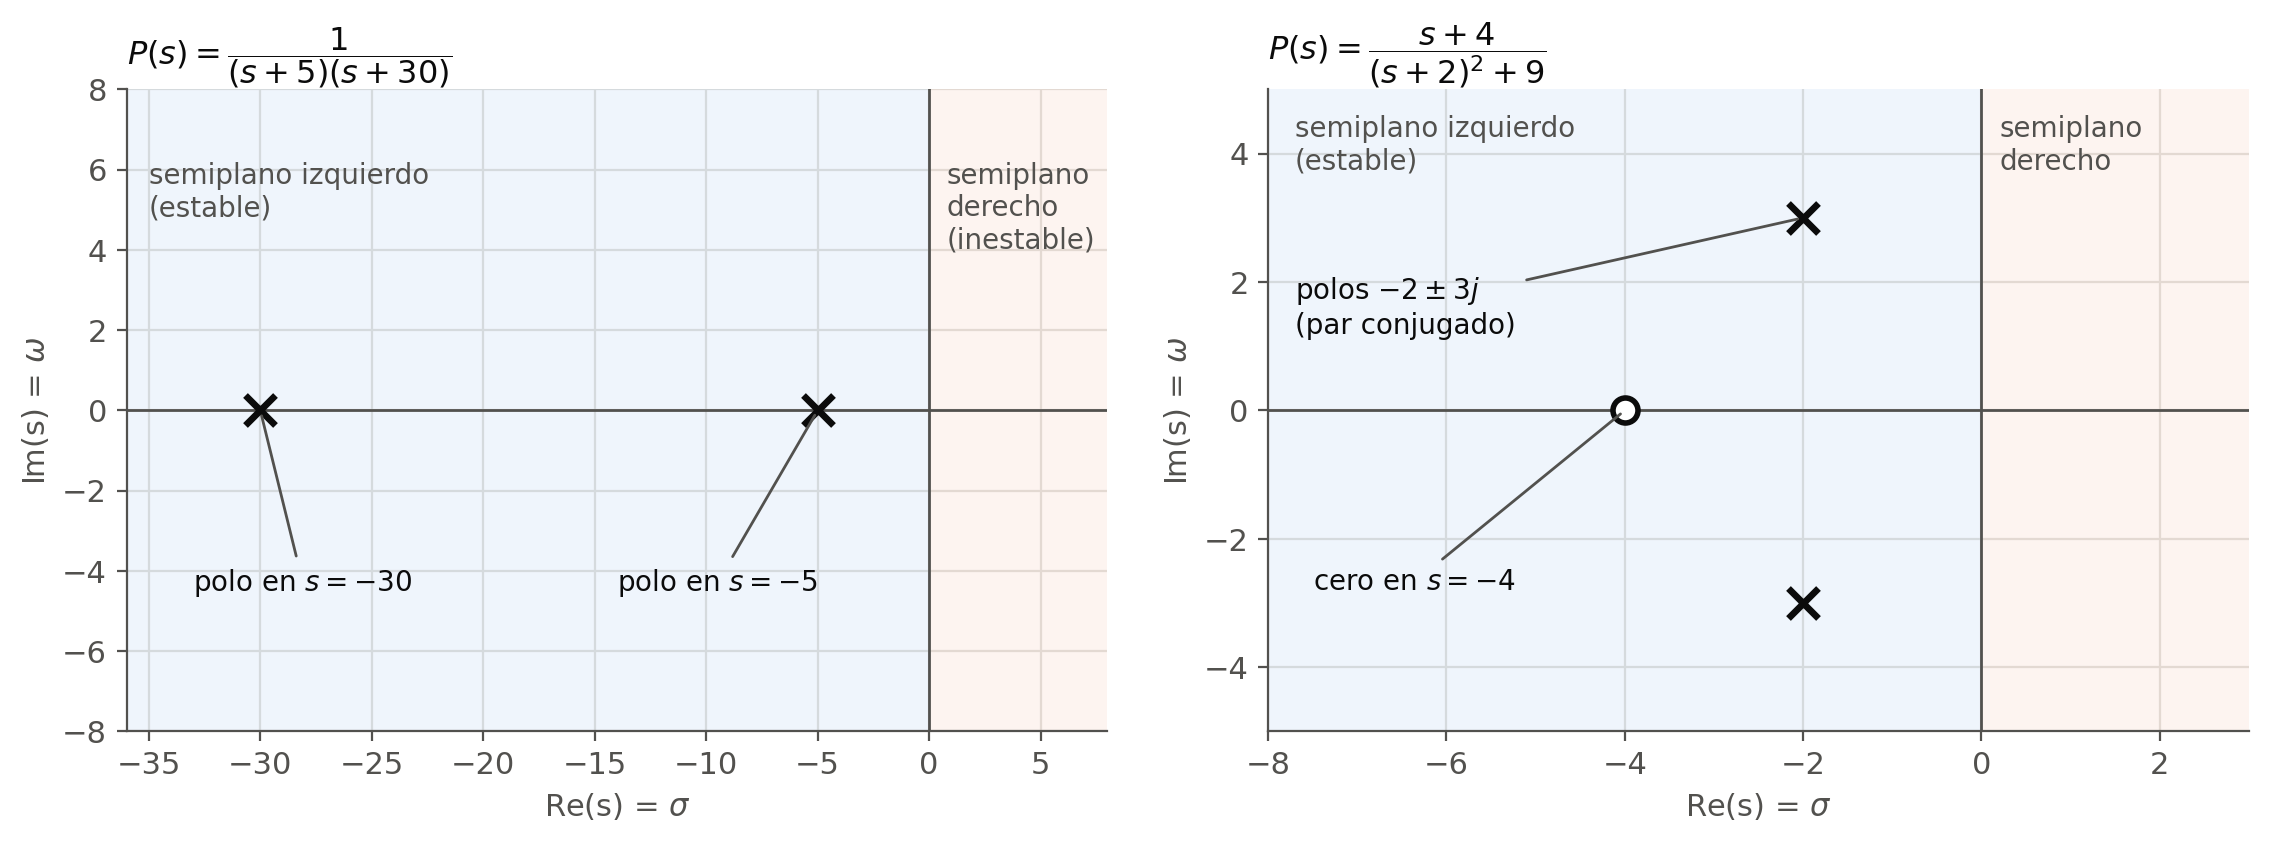
\includegraphics[width=\textwidth,height=0.66\textheight,keepaspectratio]{fig/plano_s.png}

  \smallskip
  \small $\times$ = polo, \ $\circ$ = cero. Eje horizontal: parte real $\sigma$. Eje vertical: parte imaginaria $\omega$. Los polos complejos siempre vienen en \textbf{pares conjugados}.
\end{frame}

% ------------------------------------------------------------
\begin{frame}{Qué hace cada polo: la posición decide el comportamiento}
  \centering
  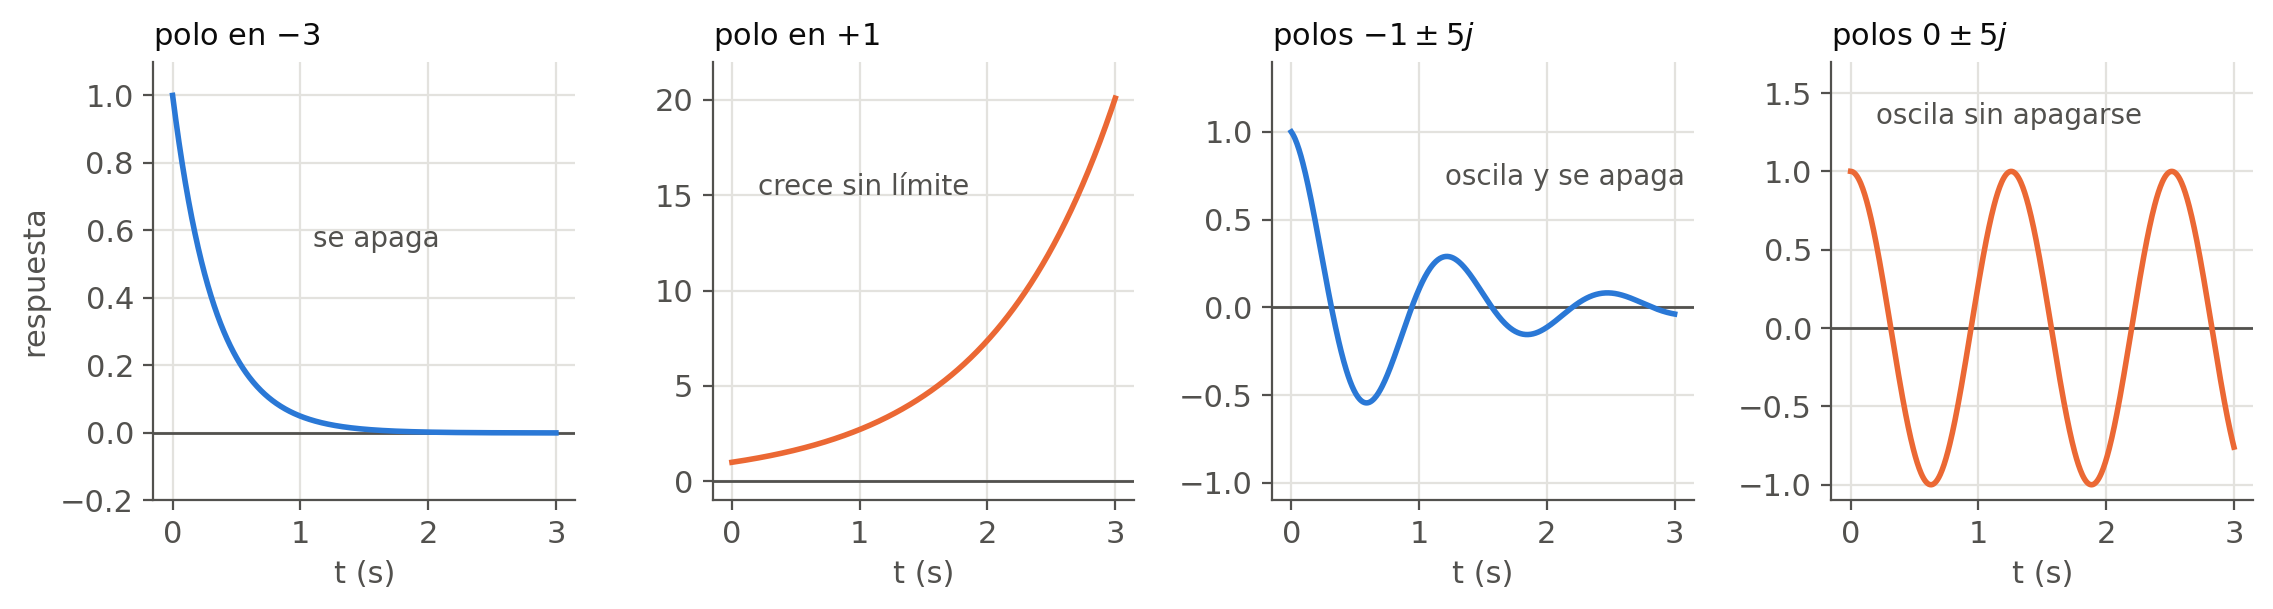
\includegraphics[width=\textwidth,height=0.52\textheight,keepaspectratio]{fig/respuestas_polos.png}

  \smallskip
  \small
  \begin{block}{Regla de estabilidad}
    Un sistema es \textbf{estable} si todos sus polos están en el semiplano izquierdo ($\operatorname{Re}(p)<0$). Un polo en el semiplano derecho hace crecer la respuesta sin límite.
  \end{block}
\end{frame}

% ------------------------------------------------------------
\begin{frame}{Evaluar $P(s)$ en $s=j\omega$: elegir un punto del eje imaginario}
  \footnotesize
  \setlength{\parskip}{1pt}
  \begin{columns}[T]
    \begin{column}{0.42\textwidth}
      \centering
      \begin{tikzpicture}[>=Stealth, scale=0.3]
        \draw[->] (-3,0) -- (3,0) node[right]{\footnotesize$\sigma$};
        \draw[->] (0,-0.5) -- (0,6.5) node[above]{\footnotesize$j\omega$};
        \foreach \w/\l in {1/1, 5/5, 10/10} {
          \pgfmathsetmacro{\y}{\w*0.6}
          \fill (0,\y) circle (2.5pt);
          \node[right] at (0.15,\y) {\footnotesize$s=j\l$};
        }
      \end{tikzpicture}
    \end{column}
    \begin{column}{0.56\textwidth}
      \begin{block}{¿Qué es $\omega$?}
        Un número \textbf{real} que elegimos: la \textbf{frecuencia} (rad/s). El punto $s=j\omega$ es el número complejo con parte real $0$ y parte imaginaria $\omega$: está sobre el eje vertical.
      \end{block}
    \end{column}
  \end{columns}

  \uncover<2->{%
  \begin{block}{Evaluar $P$ en ese punto = sustituir $s=5j$ en \emph{toda} la función}
    $P(s)=\dfrac{1}{(s+5)(s+30)}\ \Longrightarrow\ P(5j)=\dfrac{1}{(5j+5)(5j+30)}=\dfrac{1}{(5+5j)(30+5j)}$\\
    $5+5j$ y $30+5j$ son el \emph{valor} de cada factor en $s=5j$, no polos (los polos siguen siendo $-5$ y $-30$). Falta \textbf{operar}: multiplicar los dos factores y dividir (paso 1), que da $P(j5)=0.00465\,\angle{-54.46^\circ}$.
  \end{block}}

  \uncover<3->{%
  \begin{alertblock}{Recorrer}
    Al cambiar $\omega$ (1, 5, 10, \dots) el punto \emph{sube} por el eje y sale un $P(j\omega)$ distinto: es la \textbf{respuesta en frecuencia} (paso 3).
  \end{alertblock}}
\end{frame}

% ------------------------------------------------------------
\begin{frame}{¿Para qué sirve $P(j5)$? Qué hace el sistema con una senoidal}
  \centering
  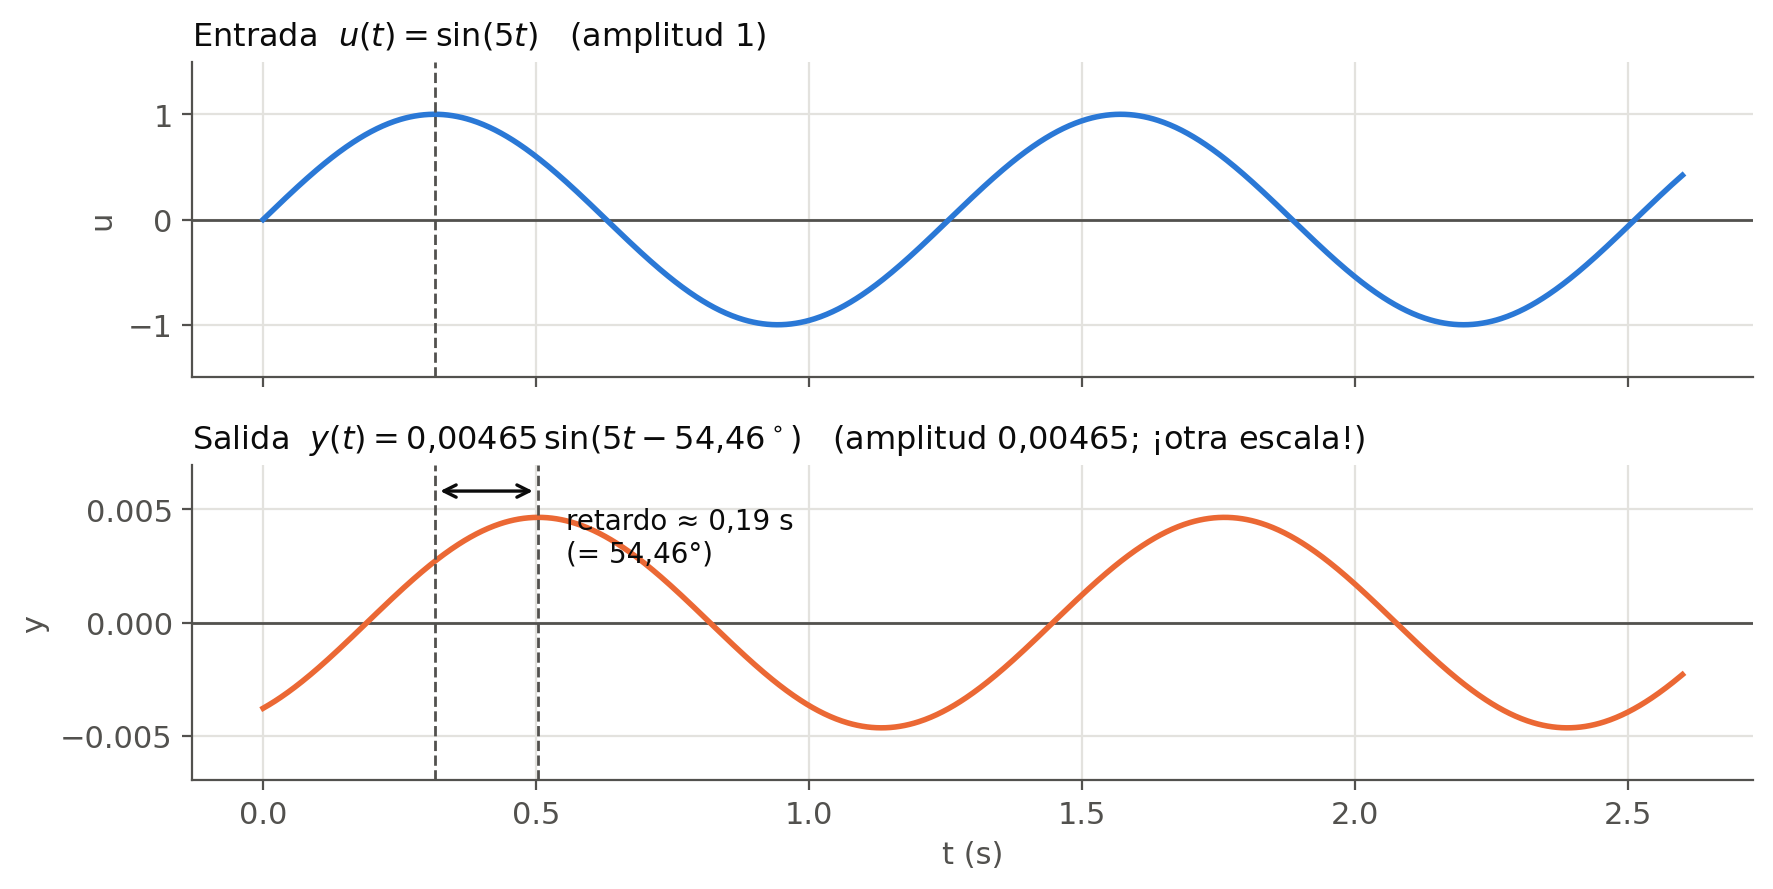
\includegraphics[width=0.9\textwidth,height=0.56\textheight,keepaspectratio]{fig/senoidal_P5.png}

  \smallskip
  \footnotesize
  \begin{block}{$P(j\omega)$ = respuesta a una senoidal de frecuencia $\omega$ (régimen permanente)}
    \textbf{Magnitud} $|P(j5)|=0.00465$ ($-46.65$\,dB): la salida es $0.00465$ veces la entrada. \textbf{Fase} $-54.46^\circ$: va retrasada.\\
    Repitiendo con otras $\omega$ se obtiene la \textbf{respuesta en frecuencia} (paso 3), y con ella el Nichols chart y los templates de QFT.
  \end{block}
\end{frame}

% ------------------------------------------------------------
\begin{frame}{Cada factor es una flecha: del polo al punto $j\omega$}
  \small
  \setlength{\parskip}{3pt}
  Restar dos números complejos da el \textbf{vector} que va del segundo al primero. Así, $(j\omega-p)$ es la flecha que va del polo $p$ al punto $j\omega$.

  \begin{columns}[T]
    \begin{column}{0.58\textwidth}
      \centering
      \begin{tikzpicture}[>=Stealth]
        \def\u{0.17}
        \draw[->] (-31*\u,0) -- (3*\u,0) node[right]{\footnotesize$\sigma$};
        \draw[->] (0,-0.4) -- (0,1.6) node[above]{\footnotesize$j\omega$};
        \node at (-30*\u,0) {\large$\times$};
        \node at (-5*\u,0) {\large$\times$};
        \node[below] at (-30*\u,-0.05) {\footnotesize$p=-30$};
        \node[below] at (-5*\u,-0.05) {\footnotesize$p=-5$};
        \fill (0,5*\u) circle (2pt);
        \node[right] at (0.1,5*\u+0.15) {\footnotesize$s=j5$};
        \draw[->, thick, blue!70!black] (-5*\u,0) -- (0,5*\u);
        \draw[->, thick, orange!85!black] (-30*\u,0) -- (0,5*\u);
      \end{tikzpicture}
    \end{column}
    \begin{column}{0.4\textwidth}
      \textcolor{blue!70!black}{\textbf{Flecha azul}}\\
      $j5-(-5)=5+5j$\\
      distancia $7.07$, ángulo $45^\circ$

      \medskip
      \textcolor{orange!85!black}{\textbf{Flecha naranja}}\\
      $j5-(-30)=30+5j$\\
      distancia $30.41$, ángulo $9.46^\circ$
    \end{column}
  \end{columns}

  \begin{block}{Qué leer en cada flecha (paso 1)}
    \textbf{Magnitud} de $(j\omega-p)$ = \textbf{longitud} de la flecha. \quad \textbf{Ángulo} = dirección de la flecha, medida desde el eje real positivo.
  \end{block}
\end{frame}

% ------------------------------------------------------------
\begin{frame}{Ejemplo: $P(j5)$ leído sobre el plano $s$}
  \small
  \setlength{\parskip}{3pt}
  Los polos están en el \textbf{denominador}, así que su distancia \textbf{divide} y su ángulo \textbf{resta} (regla del paso 1):

  \begin{center}
    \renewcommand{\arraystretch}{1.2}
    \begin{tabular}{lrr}
      \hline
      & \textbf{Magnitud (dB)} & \textbf{Fase} \\
      \hline
      polo en $-5$: \ $1/(5+5j)$ & $-16.99$ & $-45^\circ$ \\
      polo en $-30$: \ $1/(30+5j)$ & $-29.66$ & $-9.46^\circ$ \\
      \hline
      \textbf{Total} $P(j5)$ & $\boxed{-46.65}$ & $\boxed{-54.46^\circ}$ \\
      \hline
    \end{tabular}
  \end{center}

  \begin{block}{Para recordar}
    Cada \textbf{polo} aporta \textbf{fase negativa} y resta magnitud. Es el mismo resultado del ejemplo del paso 1, ahora con interpretación geométrica.
  \end{block}
\end{frame}

% ------------------------------------------------------------
\begin{frame}{Con polos complejos: una flecha por cada polo}
  \footnotesize
  \setlength{\parskip}{1pt}
  $P(s)=\dfrac{1}{(s+2)^2+9}=\dfrac{1}{(s-p)(s-p^*)}$ \ con \ $p=-2+3j,\ p^*=-2-3j$. En $s=j5$ hay \textbf{dos flechas}, una desde cada polo:

  \begin{columns}[T]
    \begin{column}{0.5\textwidth}
      \centering
      \begin{tikzpicture}[>=Stealth, scale=0.34]
        \draw[->] (-4,0) -- (1.5,0) node[right]{\footnotesize$\sigma$};
        \draw[->] (0,-3.6) -- (0,6.0) node[above]{\footnotesize$j\omega$};
        \node at (-2,3) {\Large$\times$};
        \node at (-2,-3) {\Large$\times$};
        \node[left] at (-2,3) {\footnotesize$p$};
        \node[left] at (-2,-3) {\footnotesize$p^*$};
        \fill (0,5) circle (2pt) node[above right]{\footnotesize$j5$};
        \draw[->, thick, blue!70!black] (-2,3) -- (0,5);
        \draw[->, thick, orange!85!black] (-2,-3) -- (0,5);
      \end{tikzpicture}
    \end{column}
    \begin{column}{0.5\textwidth}
      \renewcommand{\arraystretch}{1.25}
      \begin{tabular}{lrr}
        \hline
        \textbf{Flecha} & \textbf{Magnitud} & \textbf{Ángulo} \\
        \hline
        \textcolor{blue!70!black}{$j5-p=2+2j$} & $2.83$ & $45^\circ$ \\
        \textcolor{orange!85!black}{$j5-p^*=2+8j$} & $8.25$ & $75.96^\circ$ \\
        \hline
        Producto & $23.32$ & $120.96^\circ$ \\
        \hline
      \end{tabular}
    \end{column}
  \end{columns}

  \begin{block}{Resultado}
    $P(j5)=\dfrac{1}{23.32\,\ang{120.96}}=0.0429\,\ang{-120.96}$, es decir, \textbf{$-27.36$ dB y $-120.96^\circ$}. Comprobación: $(2+5j)^2+9=-12+20j$.
  \end{block}
\end{frame}

% ------------------------------------------------------------
\begin{frame}{Un cero hace lo contrario}
  \small
  \setlength{\parskip}{3pt}
  Añadimos un cero en $s=-2$: \quad $P(s)=\dfrac{s+2}{(s+5)(s+30)}$. El factor $(5j+2)$ está en el \textbf{numerador}: su distancia \textbf{multiplica} y su ángulo \textbf{suma}.

  \begin{center}
    \renewcommand{\arraystretch}{1.2}
    \begin{tabular}{lrr}
      \hline
      & \textbf{Magnitud (dB)} & \textbf{Fase} \\
      \hline
      cero en $-2$: \ $(2+5j)$ & $+14.62$ & $+68.20^\circ$ \\
      polo en $-5$ & $-16.99$ & $-45^\circ$ \\
      polo en $-30$ & $-29.66$ & $-9.46^\circ$ \\
      \hline
      \textbf{Total} $P(j5)$ & $\boxed{-32.03}$ & $\boxed{+13.74^\circ}$ \\
      \hline
    \end{tabular}
  \end{center}

  \begin{block}{Regla}
    Polo: \textbf{resta} fase y magnitud. \ Cero: \textbf{suma} fase y magnitud. \ Este reparto es la base del \textbf{diseño del controlador} (pasos 5 a 9).
  \end{block}
\end{frame}

% ------------------------------------------------------------
\begin{frame}{Ejercicio}
  Sea \quad $P(s)=\dfrac{10\,(s+1)}{(s+2)(s+20)}$
  \begin{enumerate}
    \item Indica sus polos y sus ceros y dibújalos en el plano $s$.
    \item ¿Es estable? Justifícalo.
    \item Calcula $P(j2)$: magnitud en dB y fase, sumando la contribución de cada factor (cero, polo, polo).
    \item Comprueba el resultado multiplicando en rectangular.
  \end{enumerate}
  \vspace{4pt}
  \begin{block}{Para pensar}
    ¿Qué le pasaría a la estabilidad si el factor $(s+2)$ fuera $(s-2)$?
  \end{block}
\end{frame}

% ------------------------------------------------------------
\begin{frame}{Para programarlo: el notebook de este paso}
  \small
  Todo lo de este paso se puede \textbf{ejecutar} en el notebook \texttt{notebooks/paso02\_funciones\_transferencia.ipynb}.
  \begin{itemize}
    \item Python: una clase \texttt{FuncionTransferencia}, \texttt{np.roots}, estabilidad con \texttt{all(...)}, y la respuesta a una senoidal contrastada con \texttt{scipy.signal.lsim}.
    \item Cada cálculo a mano de las diapositivas se \textbf{comprueba} en código.
    \item Incluye celdas \emph{Tu turno} con el ejercicio del paso y la solución plegada.
  \end{itemize}
  \footnotesize Requisitos: \texttt{numpy}, \texttt{matplotlib} y, en el paso 2, \texttt{scipy}.
\end{frame}

\begin{frame}{Resumen}
  \begin{itemize}
    \item La ecuación diferencial se vuelve álgebra con Laplace: \textbf{derivar $=$ multiplicar por $s$}.
    \item $P(s)=Y(s)/U(s)$ es un cociente de polinomios en $s$.
    \item \textbf{Ceros:} raíces del numerador. \textbf{Polos:} raíces del denominador, reales o complejos (estos, en pares conjugados). Un polo $p$ es el factor $(s-p)$; $(s+a)$ es un polo real en $-a$.
    \item \textbf{Estable} $\iff$ todos los polos en el semiplano izquierdo.
    \item $P(s)$ se dibuja en el plano complejo: polos y ceros son puntos ($\times$, $\circ$ son solo marcas).
    \item $P(j\omega)$: $P(s)$ sobre el eje imaginario. Magnitud $=$ distancias, ángulo $=$ direcciones.
    \item Polo: resta magnitud y fase. Cero: las suma.
  \end{itemize}
  \vspace{6pt}
  \begin{block}{Siguiente paso}
    Paso 3: respuesta en frecuencia, es decir, $P(j\omega)$ para todo $\omega$.
  \end{block}
\end{frame}

\appendix
% ------------------------------------------------------------
\begin{frame}
  \centering
  \vspace{1.2cm}
  {\Huge\bfseries Apéndice}
\end{frame}

% ------------------------------------------------------------
\begin{frame}{Solución del ejercicio: $P(s)=\dfrac{10(s+1)}{(s+2)(s+20)}$}
  \footnotesize
  \setlength{\parskip}{1pt}
  \begin{block}{1--2. Polos, ceros y estabilidad}
    Cero en $s=-1$. Polos en $s=-2$ y $s=-20$. Los dos polos están en el semiplano izquierdo, así que el sistema es \textbf{estable}.\\
    Si el factor fuera $(s-2)$, el polo estaría en $s=+2$ (semiplano derecho): sería \textbf{inestable}.
  \end{block}
  \begin{block}{3. $P(j2)$ factor a factor}
    $2j+1=2.236\,\ang{63.43}$ \quad $2j+2=2.828\,\ang{45}$ \quad $2j+20=20.10\,\ang{5.71}$\\
    Magnitud: $\dfrac{10\cdot2.236}{2.828\cdot20.10}=0.3933=\boxed{-8.11\ \text{dB}}$ \qquad Fase: $63.43^\circ-45^\circ-5.71^\circ=\boxed{12.72^\circ}$
  \end{block}
  \begin{block}{4. Comprobación en rectangular}
    $P(j2)=\dfrac{10(1+2j)}{(2+2j)(20+2j)}$, \quad $(2+2j)(20+2j)=40+4j+40j+4j^2=36+44j$\\
    $\dfrac{10+20j}{36+44j}=\dfrac{(10+20j)(36-44j)}{3232}=\dfrac{1240+280j}{3232}=0.3837+0.0866j$ \ $\Rightarrow$ \ $|P|=0.3933$, \ $12.72^\circ$. \textbf{Coincide.}
  \end{block}
\end{frame}

\end{document}
